
\begin{enumerate}
    \item A 10 cm long perfectly conducting wire PQ is moving with a velocity 1 cm/s on a pair of horizontal rails of zero resistance. One side of the rails is connected to an inductor L = 1 mH and a resistance \(R = 1 \Omega\) as shown in figure. The horizontal rails, L and \(R\) lie in the same plane with a uniform magnetic field \(B = 1 T\) perpendicular to the plane. If the key \(S\) is closed at certain instant, the current in the circuit after 1 millisecond is \(x \times 10^{-3} A\), where the value of \(x\) is \_\_\_.
    \begin{center}
        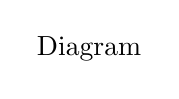
\begin{tikzpicture}
            \node {Diagram};
        \end{tikzpicture}
    \end{center}
    \item[Note:] Assume the velocity of wire PQ remains constant (1 cm/s) after key \(S\) is closed. Given: \(e^{-1} = 0.37\), where \(e\) is base of the natural logarithm.
\end{enumerate}
